\section{Recursion}

\subsection{Factorial}
A classic way of demonstrating recursion is factorial. 4! means
4 * 3 * 2 * 1.

The broken down steps can be seen below.

\begin{verbatim}
4! = 4 * 3 * 2 * 1
       12  * 2 * 1
            24 * 1
               24
4! = 24
\end{verbatim}

The \emph{factorial} function can be defined in Haskell.
If there is no base case defined, the recursion will go on forever and will never stop.

\begin{lstlisting}
fac :: Integer -> Integer
fac 0 = 1 -- base case
fac n = n * fac (n -1)
\end{lstlisting}

\footnote{\emph{fac 0 = 1} is the base case since it will return 1, and stop the recursion.}

\subsection{More examples of recursion}
Some more examples of recursion from \emph{work/recursion.hs}.

\lstinputlisting[breaklines]{work/recursion.hs}

\newpage
\subsection{Foldl vs foldr style recursion}
\emph{foldr} folds a list from right to left, whereas \emph{foldl} folds
a list from left to right.

\emph{foldl} stacks parentheses on the left where as \emph{foldr} stacks them on the right
(((0+1)+2)+3) vs (1+(2+(3+0)))

\begin{figure}[h]
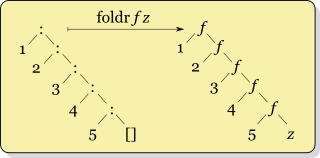
\includegraphics[width=0.7\textwidth]{foldr-rec.png}
\centering
\caption{foldr recursion}
\end{figure}

\begin{figure}[h]
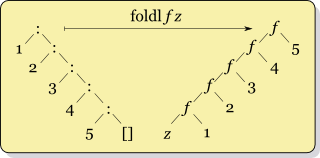
\includegraphics[width=0.7\textwidth]{foldl-rec.png}
\centering
\caption{foldl recursion}
\end
{figure}